\chapter{Methods}
\label{chap:methods}
%LM,KNN,Tree,ANN,Garch - qu'est-ce que c'est et comment ça marche

\section{\acrlong{ts} Methods}
We'll go over the various methods we will be using, giving a brief description and explaining in what cases they are used.
Unlike with regular regression, \acrlong{ts} analysis generally doesn't use auxiliary data to predict how the series will behave, but exploits intrinsic relation within the series itself. Often using some combination of previous values and randomness to predict the next value.
The data must therefore have a \acrlong{ts} representation. That is, we can index it by an ordered set, such as time.
Let us denote such a series by $\{Y_t\}_{t=1,\dots,n}$.
It is generally assumed that a \acrlong{ts} has to be stationary to work with. In other words, the series should have a constant mean, and a covariance function depending only on the lag between 2 observations (and not for example of the time step). In practice, trend is removed from the series before analysis all together and then is added back at the end if necessary.
Classic \acrlong{ts} methods are generally good at explaining \acrshort{ts}, but are less interesting for predictions, as they always predict the expected value, as we will see with our Tesla case.


\subsection{\acrshort{arma}}
\acrfull{arma} model \cite{ARMAbook} have 2 components: an \acrfull{ar} part and a \acrfull{ma} part. 
The \acrshort{ar} part, as it's name suggests, is a regression of the series with itself. That is, we suppose that an observation is a linear combination of a certain number of previous observations, plus a little noise. Here the noise of each observation has an indirect influence on following values.
The \acrshort{ma} part, on the other hand, assumes that the error terms of previous observations have a direct influence on following values. In other words, we use previous error terms as covariates to do regression on the series.
Putting both together we get the general \acrshort{arma} model.
An \acrshort{arma} (p,q) model is defined by:
$$
Y_t = \sum_{j=1}^p \phi_j Y_{t-j} + \sum_{j=1}^q \theta_j \epsilon_{t-j} + \epsilon_t
$$
Where the $\phi_j$'s and $\theta_j$'s are constants with $\phi_p , \theta_q \neq 0$. These are the parameters that have to be estimated. Usually $\epsilon_t \stackrel{iid}{\sim} \mathcal{N}(0,1)$ but could be any distribution with zero mean and unit variance.

\subsection{\acrshort{garch}}
\label{subsec:garch}
\acrshort{arma} models make an assumption that can be quite limiting for financial \acrlong{ts}, in that it assumes the variance is homogeneous throughout time, but with financial data this is practically never the case. There are always periods of more volatility than other, for example when there is a big announcement or a scandal, or other speculative uncertainty. 
To address this problem, a model was developed for modeling noise in a \acrlong{ts} that was variable: the \acrfull{arch} model \cite{ARCHpaper}, and later it's generalization, the \acrfull{garch} model \cite{GARCHpaper}.

The idea of these models, is to model the variance as an \acrshort{arma} process. This leads to the following definition.

A \acrshort{garch}(m,r) model is defined by:
$$
Y_t = \sigma_t \epsilon_t
$$
$$
\sigma_t^2 = \alpha_0 + \sum_{j=1}^m \alpha_j Y_{t-j}^2 + \sum_{j=1}^r \beta_j \sigma_{t-j}^2
\quad, \epsilon_t \stackrel{iid}{\sim} F(0,1)
$$
where $F$ is any distribution with zero mean and unit variance. Often it is either Normal or Student t (that has been standardized).
\acrshort{garch} models are generally the \acrlong{ts} models used for financial data, but more generally it is used any time the variance is clearly not constant. A \acrshort{garch} model can also be combined with an \acrshort{arma} model, to create and \acrshort{arma}-\acrshort{garch} model. As we will see later on, this will not be necessary here so we will not go further into these models.

\section{\acrshort{ml} Methods}
We'll go over the various methods we will be using, giving a brief description and overview of the pros and cons of each and when it is appropriate to use them.
Following the same notation as in chapter \ref{chap:experiment_design}, let $(\mathcal{X},\mathcal{Y})$ denote the features and responses of our data. A \acrshort{ml} model is some function that takes the features $\mathcal{X}$ as inputs and returns an approximation of the responses $\hat{\mathcal{Y}}$ as output. Let us denote a generic model by $F$ in such way that $\mathcal{Y} \approx \hat{\mathcal{Y}}=F(\mathcal{X})$.
The goal of \acrshort{ml} is to find methods that give good approximating functions $F$. The two questions that arise are "What do we use as approximating function $F$ ?" and "What makes an approximation 'good' ?". The second question was addressed in the previous chapter when discussing error measures. We will tackle the first question now. In the following we shall explore various methods (models $F$) that have been developed.

First, however, as we are dealing with finite sets, we will suppose that there are $n$ observations and $m$ features. In this section we will only specify the methods for the univariate response case, and not go into details about the generalization to multivariate responses. This all allows us to rewrite the above sets as:
$$\mathcal{X}=\{(X_{i1},\dots,X_{im}) : i=0,\dots,n\}$$
$$\mathcal{Y}=\{Y_i : i=0,\dots,n\}$$
$$\hat{\mathcal{Y}}=\{\hat{Y}_i : i=0,\dots,n\}$$
And the model relation as:

$$
Y_i \approx \hat{Y}_i = F(X_{i1},\dots,X_{im}) \quad \forall i \in \{1:n\}
$$

For simplicity in notation, we will often use $ \vec{X_i}=(X_{i1},\dots,X_{im}) $. We are now ready to explore the first method.

\subsection{\acrlong{lm}}
The idea is to use a linear combination of features to determine the response. The linear constants are the parameters that need to be chosen to give the best approximation of the response space using the feature space. Geometrically this means fitting a hyperplane to the training set, by minimizing some function (loss function).
Formally:
$$
\hat{Y}_i = \sum_{j=1}^m \beta_{j} X_{ij} \quad, i=1,\dots,n
$$

\subsubsection{Advantages}
\begin{itemize}
\item Very well understood
\end{itemize}

\acrlong{lm} are some of the most common and simple models out there, but they have proven to be reliable and can be made quite complex with feature engineering. There is plenty of theory and proofs about these methods. This all makes these methods and obvious first choice of methods to consider.
%insert "toute est linéaire" quote
\subsubsection{Problems}
\begin{itemize}
\item Linearity assumption
\end{itemize}
Assumes that the outputs are a linear combination of quantities. Although the fact that the linearity is in the parameters leaving a lot of room for complexity with feature engineering (like for example adding an artificial feature that is the square of another feature), this is still limiting as not all relations between the data can be expressed.
\begin{itemize}
\item Suffers from multicolinearity 
\end{itemize}
In it's basic form, \acrlong{lm} uses \acrfull{ols} which assumes the features are independent. If some are highly colinear, the method becomes unstable and small random errors in the observations will produce a large impact, thus increasing the variance. This problem can be addresses partially by regularization (or shrinkage): putting a penalty on the size of the parameters. Example of this are Ridge and Lasso regression.

\subsection{K Nearest Neighbours}
The intuition behind \acrfull{knn} methods is simple. The idea is that observations (points in the feature space) which are "close" will have responses that are also "close". Then a good approximation would be given by averaging the responses of the K observations "closest" to the new observation.
In this model, we need to chose the definition of "close" as well as chose the value of K.

Formally:
 $$
 F(\vec{X_+}) = 1/K \sum_{i:\vec{X_i} \in N(X_+)}^{Y_i}
 $$

Where the neighborhood $N(\vec{X_+})$ of $ \vec{X_+} $ is the collection of $K$ closest observations

Usually, the distance used to define "close", is the euclidean distance and that is the one we used. As for K, this parameter needs to be tuned. The larger it is the smoother the result is and the lower the more jagged it is. For optimal tuning the parameter should be as small as possible, without over-fitting.
\subsubsection{Advantages}
\begin{itemize}
\item Intuitive
\end{itemize}
The concept is very simple to understand, we are just taking the average of a new point neighbors to determine the output
\begin{itemize}
\item Simple to implement
\end{itemize}
It takes only a few lines of code to implement \acrshort{knn} and get it up and running.
\begin{itemize}
\item Non parametric
\end{itemize}
No prior knowledge about how the data is actually distributed is made, which makes it a flexible tool that can be used anywhere.

\subsubsection{Problems}
\begin{itemize}
\item Curse of dimensionality 
\end{itemize}
It suffers from curse of dimensionality. When the dimension of the feature space gets large, the space becomes sparsely populated, and the K closest observations, might actually be very far from each other, and thus not reflect well the new observation.
As a workaround for this problem, there is a variant of \acrshort{knn} which instead of using the K closest observations, uses all the observations which fall in a certain radius of the new observation point. Thus the K parameter becomes R, the radius of the hyperball. A problem with this version is that there may be no observations that fall in the hyperball of a new data point and then nothing can be inferred about it.
\begin{itemize}
\item Piecewise constant
\end{itemize}
The response space is discretized so not all outcomes can be predicted.

\subsection{Trees}
To understand more sophisticated tree methods, we first need to understand how a simple tree works for regression. In \acrshort{knn}, the feature space in separated into regions (or "strats") and fits a constant to each region. A \acrfull{dt} \cite{DTpaper} works much the same way, but allows for different and more complex definitions of strats.
A simple binary tree, or a \acrshort{dt}, works by splitting the feature space recursively into simple strats. Each leaf of the tree corresponds to a strat and the constant is the average of all observations that correspond to that leaf. A fully grown tree, i.e. where each observation corresponds to one leaf exactly, is equivalent to 1-NN.
 Once a tree has been grown, the predictor $\hat{Y}_i$ of $\vec{X_i}$ is the average of all the $Y_i$ in the strat that $\vec{X_i}$ falls into. The prediction function is therefore piecewise constant.
Formally:
$$
F(\vec{X_i}) = \sum_{l=1}^L c_l I(\vec{X_i} \in A_l)
$$
Where there are $L$ strats denoted by $A_l$ and $c_l$ are the averaging constants.
It is NP-hard to determine the optimal Decision Tree for a given data set, and thus greedy approaches are used. Each split is determined by the variable and threshold that minimize the \acrlong{mse} of the split. A \acrshort{dt} is usually not grown out all the way, if used by itself.

\subsubsection{Advantages}
\begin{itemize}
\item Non parametric
\end{itemize}
Trees make no assumption on how the data is actually distributed and can be used on any data. Very little thought has to go into it
\begin{itemize}
\item Logarithmic complexity for prediction
\end{itemize}
Trees are inexpensive to use (once built) to predict values as they have a logarithmic complexity due to the binary splitting nature of Trees.
\begin{itemize}
\item Easy to understand
\end{itemize}
The concept of \acrlong{dt} are very simple and they can be visualized, which helps to understand them.
\subsubsection{Disadvantages}
\begin{itemize}
\item High variance
\end{itemize}

The choice of each split, especial the first ones, can greatly influence the outcome of the model and thus \acrshort{dt} have high variance.

\begin{itemize}
\item Over-fitting is easy
\end{itemize}
If we grow the Tree out completely, we will end up with a model where every leaf explains exactly one observation. This is a case of extreme overfitting, but even if we stop earlier we can easily over fit if the stopping criteria is not well decided.
\begin{itemize}
\item Unstable
\end{itemize}
A tree could look completely different if the first split is different or any subsequent split is different (but with decreasing impact). This means Trees are unstable; a slight change in the data might completely change the outcome.
\begin{itemize}
\item No optimality
\end{itemize}
In theory there exists an optimal \acrshort{dt}, but the problem of finding the optimal Tree is NP-hard, so in practice we use a greedy algorithm to grow the Tree. This means the final Tree might not be close to the optimal tree at all.
\begin{itemize}
\item Not smooth
\end{itemize}
The model is piecewise constant, and so the prediction space is not smooth.


The variations of \acrlong{dt} we shall consider are

\begin{description}
\item [\acrfull{rf} \cite{RFpaper}] work by taking many \acrlong{dt} constructed by taking random samples of the training set, with replacement, and then averaging the trees. At each split a random number of variables are chosen, thus ensuring that if a variable is predominant, it won't always be chosen first in each tree of the forest, thus decreasing the correlation of the trees amongst themselves and in turn increasing the reduction in variance.
This will reduce the variance, with a cost of raising the bias a little.

\item [\acrfull{et} \cite{ETpaper}] are random forests, but in each tree, the split is determined by a random threshold, decreasing even more the correlation of trees. 
Again this leads to less variance but a slightly higher bias
\end{description}


\subsection{\acrlong{ann}}
A fully in-depth and formal explanation of Neural Networks would take us out of the scope of this report. The literature on the subject is immense and the idea dates back to the 1950's and has grown ever since. As such we will give only a brief and simplified explanation in this report.
The idea behind \acrfull{ann} is to try to imitate the way neurons work in a brain: the neurons are connected together in a complex network, and when they are stimulated by inputs enough to reach a certain activation level, they will transmit a signal to certain neighboring neurons, combining signals, and so forth until some output is produced.

\begin{figure}
	\centering
	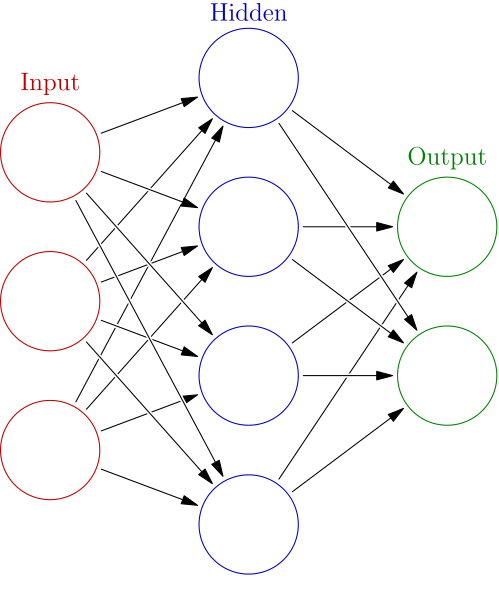
\includegraphics[width=0.5\textwidth]{img/Colored_neural_network.png}
	\caption{Schematic of an \acrlong{ann} source from \url{https://en.wikipedia.org/wiki/Artificial_neural_network}}
	\label{fig:nn}
\end{figure}

An \acrshort{ann} consists of an input layer, and output layer and multiple hidden layers (see Figure \ref{fig:nn}). The inputs are linearly combined, if activated, into the next layer of neurons, which is combined again, and again until reaching the output layer.

\subsubsection{Advantages}
\begin{itemize}
\item Can learn non-linear models
\end{itemize}
The models can be used on a wide variety of problems, including those which have non-linear properties, and if tuned right work relatively well. A lot of people don't even think too much about the regression problem they have and just throw a Neural Network at it.

\subsubsection{Problems}
\begin{itemize}
\item Non-convex loss function
\end{itemize}
This might lead to multiple local minimum, and a different random weight initialization can lead to very different results

\begin{itemize}
\item Hyperparameters tuning
\end{itemize}
There are a lot of parameters to tune, such as the number of hidden layers, the size of each hidden layer, what activation function to use, what L2 penalization, etc.
\begin{itemize}
\item Sensitive to feature scaling
\end{itemize}
If some features are not scaled the same as others, they may dominate or be dominated in the output, rendering a portion of the features useless.
\begin{itemize}
\item Black box
\end{itemize}
There is no interpretability of the relation between the inputs and outputs. The model just does it's thing and spits out a result.